\chapter{検証ライブラリActario}
\label{chapter:overview}

Actario\cite{Yasutake:2015aa}とは,本研究で作成したアクターシステムの検証用ライブラリである.
ActarioはGitHub\footnote{分散バージョン管理システムGitを利用したソースコードホスティングサービス}で公開されている\footnote{\url{https://github.com/amutake/actario}}.
Actarioは,(1) アクターシステムを記述するための型と記法,(2) アクターシステムの仕様を記述するための関数,(3) アクターシステムが仕様を満たすことを証明するためのタクティク,(4) 記述したアクターシステムをErlangに変換するための抽出機構,の4つを持っている.
本章では,階乗を計算するアクターシステムについてActarioの概要と利用方法について説明していく.

\section{概要}

図\ref{img:overview:workflow}は,Actarioを用いてアクターシステムを検証する際のワークフローである.
ActarioのユーザーはまずActarioが提供するアクターシステムを記述するための記法を使って,検証したいアクターシステムを記述する.
次にそのアクターシステムが満たしているべき仕様を記述し,それをActarioが提供するアクターモデルの意味論と証明の機構によって証明する.
最後にActarioが持つErlangへのコード抽出機を用いて実装をErlangに抽出する,という流れになる.

\begin{figure}[tp]
  \centering
  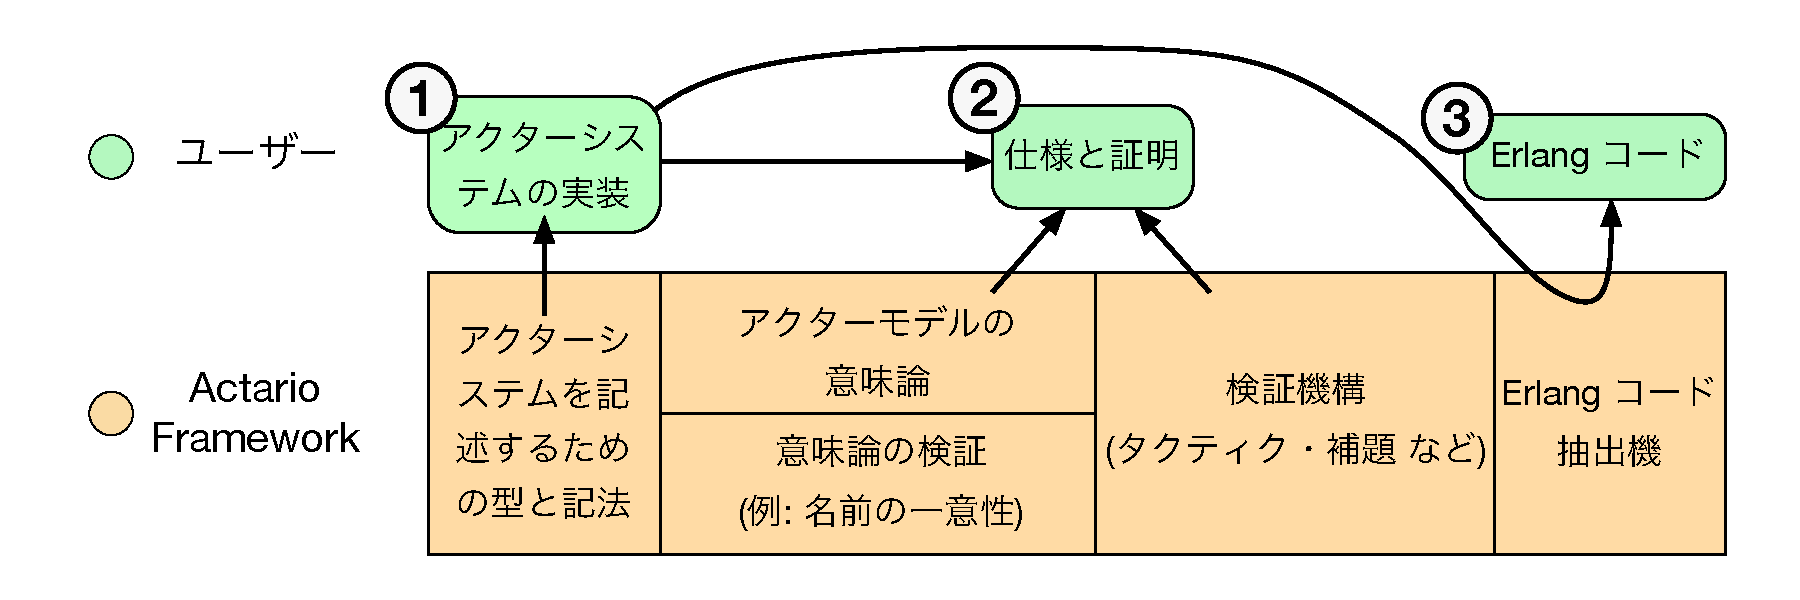
\includegraphics[width=15cm]{./img/overview/workflow.pdf}
  \caption{Actarioのワークフロー}\label{img:overview:workflow}
\end{figure}

\section{例:階乗計算アクターシステム}

例として,階乗を計算するアクターシステムを考える.
このシステムをActarioで記述し,仕様および証明を記述することで,
Actarioを実際にどのように使うかを説明する.

\subsection{システムの実装}

階乗は再帰関数の形で実装することが多いが,今回は例のためアクターを生成しメッセージパッシングを行う形で実装する.
このアクターシステムは,単に一つのアクターのなかで階乗を計算するのではなく,
「次に何を掛けるか」という継続を持っているアクターを生成していき,
継続を持っているアクターが数珠つなぎのようにメッセージを送信することで,階乗を計算する.

図\ref{img:overview:fact}はこのアクターシステムに$3$を与えたとき,つまり$3!$を計算するときのシステムの動きを表した図である.
実線の矢印はメッセージの送信を表し,破線の矢印はアクターの生成,そして縦の線は各アクターの時系列を表している.

\begin{figure}[tp]
  \centering
  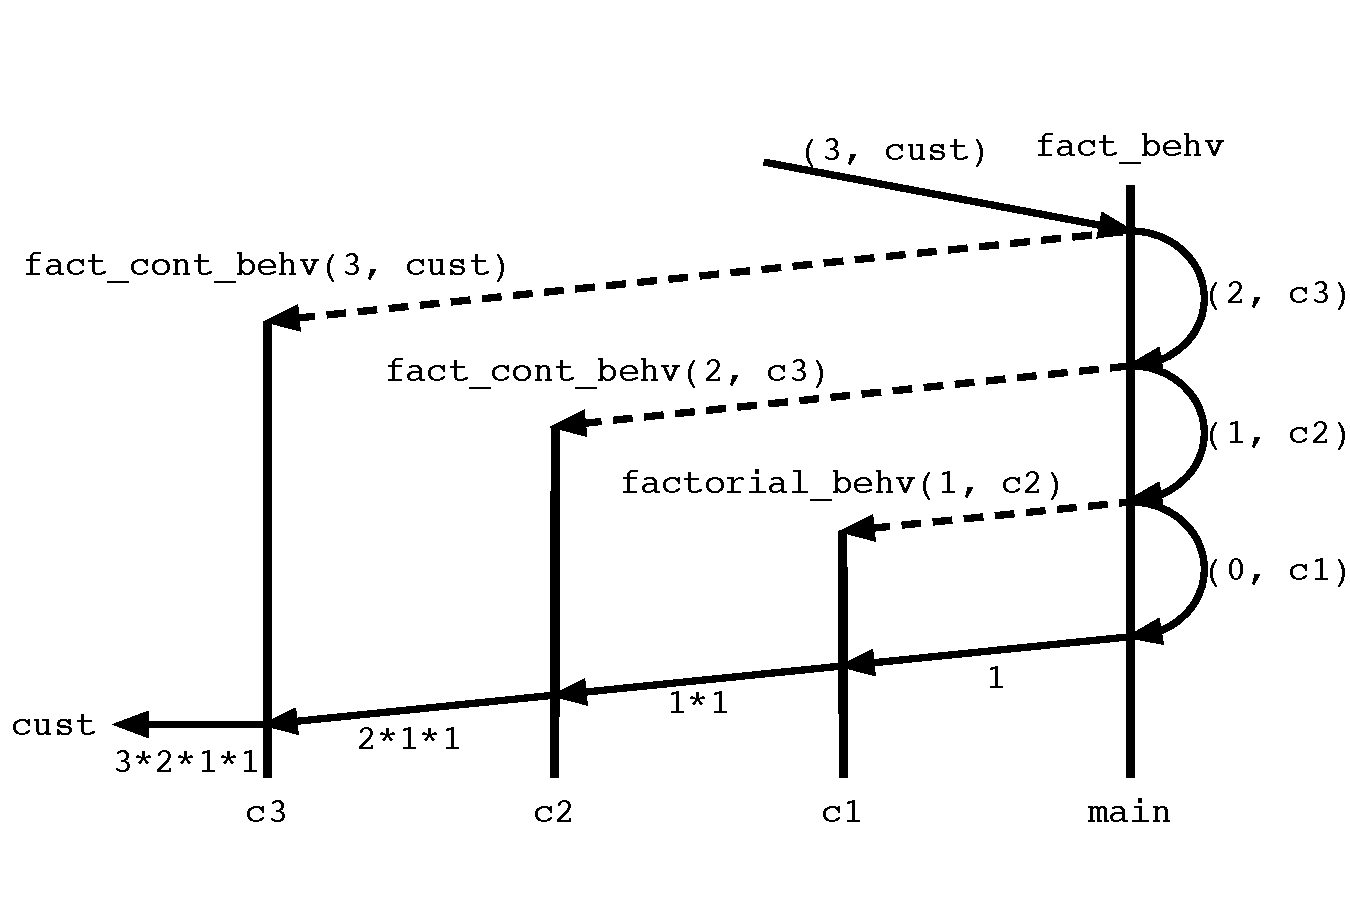
\includegraphics[width=15cm]{./img/overview/fact.pdf}
  \caption{$3!$を計算する際のシステムの動き}\label{img:overview:fact}
\end{figure}

Actarioを用いると階乗計算アクターシステムは図\ref{code:overview:fact-impl}のように記述することができる.以下でコードの説明を行う.

まず\coqi{ContState}は継続を表すアクターが保持している内部状態を表す型である.
\coqi{val_cust}と\coqi{cont_done}の2つの値コンストラクタがあり,
\coqi{val_cust}は次に掛ける自然数と掛けたあとに送信する先のアクターの名前を持っているということを,
\coqi{cont_done}は計算し終えたことを表している.

\coqi{factorial_cont_behv}は継続を保持しているアクターの振る舞いのテンプレート(内部状態を受け取り振る舞いになるような関数)である.
保持する数と計算結果を渡すアクターの名前を受け取り,アクターの振る舞いとなる.
このアクターは,メッセージを受け取った際にそれが数なら保持している数(\lstinline{val_cust} の第一引数)と掛けあわせ,
計算結果を待ち受けているアクター(\lstinline{val_cust} の第二引数)に送信する.
送信後の内部状態は\coqi{cont_done}に変更され何もしないアクターとなる.

\coqi{factorial_behv}は,継続となるアクターを次々と生成していくアクターの振る舞いのテンプレートである.
このアクターは,メッセージとして受け取った自然数が$0$の場合と$1$以上の場合でメッセージの処理が異なる.
まず$1$以上の数を受け取った場合は,前述した継続となるアクターの振る舞いテンプレートから初期状態を受け取った数と受け取った名前でアクターを生成し,次に数を$1$減らした数と生成した名前を自分自身に送信する.これを$0$を受け取るまで繰り返すことで,$n, n - 1, \cdots, 2, 1$ という数を保持するアクターを作っていく.
次に受け取った数が$0$の場合は,継続アクターを生成していれば直前に生成した継続アクター,つまり$1$を保持している継続アクターに$1$を送信し,継続アクターを生成していない,つまり$0!$を計算することを要求されていたならば,階乗の計算結果を送信するアクターに向けて$1$を送信する.

最後の\coqi{initial_actions}と\coqi{factorial_system}はこのアクターシステムを起動する部分である.\coqi{factorial_system}の\coqi{init}の第一引数はこのシステムの名前で,第二引数ははじめに実行するアクションの列である.

\begin{figure}[tp]
  \lstinputlisting{./code/overview/fact_impl.v}
  \caption{階乗計算アクターシステム}\label{code:overview:fact-impl}
\end{figure}

\subsection{型と記法}

Actarioを用いてアクターシステムを記述する際に使う型およびアクションの記法について簡単に説明する.
これらの型とアクションのアクターモデルの操作的意味論における意味については第\ref{chapter:formalization}章で説明する.

まず\coqi{name}はアクターの名前を表す型であり,\coqi{message}はメッセージを表す型である.
\coqi{message}は図\ref{code:overview:message}のように定義されている.Actarioでは空のメッセージ,名前,文字列,自然数,ブール値,そしてメッセージの組をアクター間でやりとりするメッセージとすることができる.

\begin{figure}
  \lstinputlisting{./code/overview/message.v}
  \caption{\coqi{message}型の定義}\label{code:overview:message}
\end{figure}

\coqi{behavior}はアクターの振る舞い,つまりメッセージを受け取ってどのような処理をするかを表すような型である.
\coqi{behavior}型は図\ref{code:overview:behavior}のように定義されている.
\coqi{behavior}は厳密には型コンストラクタであり,型コンストラクタの引数はその振る舞いの内部状態を表す型である.ここでは\coqi{behavior}型コンストラクタが状態を表す型を受け取り具体型となったものの意として\coqi{behavior}型と呼ぶ.
そして\coqi{receive}は\coqi{behavior}の値コンストラクタである.メッセージを受け取ってアクションの列を返すような関数を受け取って,\coqi{behavior}になる.

\begin{figure}
  \lstinputlisting{./code/overview/behavior.v}
  \caption{\coqi{behavior}型の定義}\label{code:overview:behavior}
\end{figure}

Actarioではアクターモデルのアクションとして\coqi{new},\coqi{send},\coqi{self},\coqi{become}があり,これらは\coqi{actions}型の値コンストラクタとなっている.
\coqi{actions}型はアクションの列を表しており,図\ref{code:overview:actions}のように定義されている.
\coqi{new}はアクターを生成するアクションである.振る舞いのテンプレート,初期状態,そして生成したアクターの名前を受け取って残りのアクションの列になるような継続となる関数を受け取る.
\coqi{send}はメッセージを送信するアクションである.送り先の名前と送りたいメッセージと残りのアクションの列を受け取る.
\coqi{self}は自分自身の名前を得るためのアクションである.自分自身の名前を受け取って残りのアクションの列になるような継続と成る関数を受け取る.
\coqi{become}は自分自身の状態を引数として受け取った状態に変え,次のメッセージの待ち状態になるアクションである.\coqi{become}のみ,残りのアクションの列を受け取らないのは,アクションの列の最後は必ず\coqi{become}になるようにするためである.

\begin{figure}
  \lstinputlisting{./code/overview/actions.v}
  \caption{\coqi{actions}型の定義}\label{code:overview:actions}
\end{figure}

このように,アクションの列は継続渡しの形で定義されている.アクションを記述する際には,通常のCoqの構文のとおりに記述しても良いが,煩雑になるため,CoqのNotation機能を使って図\ref{code:overview:notation}のように記述できるようにしている.

\begin{figure}\centering
\begin{minipage}{0.42\textwidth}\centering
\begin{lstlisting}[frame=single,numbers=none,xleftmargin=0pt]
new $tmpl$ $ini\_state$ (fun x =>
  self (fun s =>
    send x (name_msg s)
      (become $new\_state$)))
\end{lstlisting}
(a) 記法を用いない場合
\end{minipage}
\hspace*{3ex}
\begin{minipage}{0.42\textwidth}\centering
\begin{lstlisting}[frame=single,numbers=none,xleftmargin=0pt]
x <- new $tmpl$ with $ini\_state$;
s <- self;
x ! (name_msg s);
become $new\_state$
\end{lstlisting}
(b) 記法を用いる場合
\end{minipage}
\caption{アクションの記法の使用例}\label{code:overview:notation}
\end{figure}


\subsection{命題の定義と証明}

以上で階乗を計算するアクターシステムを記述できたが,ここではこのアクターシステムが階乗を計算するかどうかを確かめるために,「このアクターシステムは3の階乗を計算する」という命題を証明する.
命題は図\ref{code:overview:fact-spec}のように記述することができる.これは,$3$を階乗計算システムに送信し結果を\coqi{top}というアクターに送るようにすると,\coqi{top}というアクターはいつか$3! (= 6)$を受け取るという意味である.

\begin{figure}[tp]
\begin{lstlisting}
Theorem receive_3 :
  eventually_receive (factorial_system 3 top) top (nat_msg 6).
\end{lstlisting}
\caption{命題の定義}\label{code:overview:fact-spec}
\end{figure}

そして,この命題は図\ref{code:overview:fact-proof}のように証明することができる.
行っていることとしては,このアクターシステムの遷移を一つずつ追っていき,\coqi{top}が$6$を受け取るような遷移を見つけるというものである.遷移できなくなるまで遷移の生成はActarioが提供するタクティクが行う.
使っているタクティクの詳細は第\ref{chapter:proof}章で説明する.

\begin{figure}[tp]
\begin{lstlisting}
Proof.
  unfold_eventually eventually_receive=> p p0 is_path.
  step_until_stop is_path p0.
  found 22 p22 p23.
Qed.
\end{lstlisting}
  \caption{証明}\label{code:overview:fact-proof}
\end{figure}


\subsection{Erlangへのコード抽出}

ActarioはErlangへのコード抽出機構も持っているため,
定義したアプリケーションをErlangに変換して実行させることもできる.
\coqi{Extraction}コマンドではなく,図\ref{code:overview:extraction}のように\coqi{ActorExtraction}コマンドを実行すると,\coqi{factorial_behv}のErlang実装が図\ref{code:overview:fact-impl-erl}のようなコードで\texttt{factorial.erl}というファイル名で吐き出される.
これに対して,図\ref{code:overview:run}といったようなコードで変換されたアクターシステムを起動させると,実際にアクターシステムを実行することができる.

\begin{figure}[tp]
\begin{lstlisting}
ActorExtraction "factorial" factorial_behv.
\end{lstlisting}
\caption{コード抽出}\label{code:overview:extraction}
\end{figure}

\begin{figure}
  \lstinputlisting[language=Erlang]{./code/overview/fact_impl.erl}
  \caption{Erlangに抽出されたアクターシステム}\label{code:overview:fact-impl-erl}
\end{figure}

\begin{figure}
\begin{lstlisting}[language=Erlang]
-module(fact_main).
-export([fact/1]).

fact(N) ->
    FactorialActor = spawn(fun() -> factorial:factorial_behv({tt}) end),
    FactorialActor ! {tuple_msg, {nat_msg, int2nat(N)}, {name_msg, self()}},
    receive
        {nat_msg, Result} ->
            io:fwrite("fact(~w) = ~w~n", [N, nat2int(Result)]);
        _ ->
            io:fwrite("error~n")
    end.

nat2int({o}) -> 0;
nat2int({s, N}) -> nat2int(N) + 1.

int2nat(0) -> {o};
int2nat(N) when N > 0 -> {s, int2nat(N - 1)};
int2nat(_) -> {o}.
\end{lstlisting}
\caption{抽出したアクターシステムを起動するErlangコード}\label{code:overview:run}
\end{figure}
